\begin{adjustwidth*}{}{-2.25in}
\textbf{{\large Exercises}}
\setlength{\columnsep}{25pt}
\begin{multicols*}{2}
\noindent Terms and Concepts \small
\begin{enumerate}[1)]
\item Describe what an ``extreme value'' of a function is in your own words.
\item Sketch the graph of a function $f$ on $(-1,1)$ that has both a maximum and minimum value.
\item Describe the difference between and absolute and relative maximum in your own words.
\item Sketch the graph of a function $f$ where $f$ has a relative maximum at $x=1$ and $\fp(1)$ is undefined.
\item T/F: If $c$ is a critical value of a function $f$, then $f$ has either a relative maximum or relative minimum at $x=c$. 
\end{enumerate} 

\noindent {\normalsize Problems} \small

\noindent{\bf In exercises 6--7, identify each of the marked points as an absolute maximum or minimum, a local maximum or minimum, or none of the above.}

\begin{enumerate}[1),resume]
\item \begin{minipage}{\linewidth}
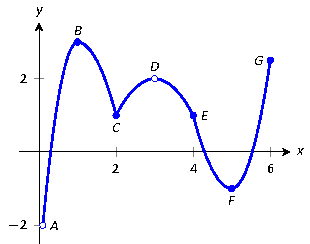
\includegraphics[scale=.8]{figures/fig03_01_ex_06}
\end{minipage}

\item \begin{minipage}{\linewidth}
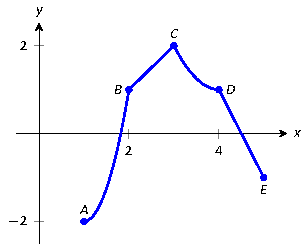
\includegraphics[scale=.8]{figures/fig03_01_ex_07}
\end{minipage}
\end{enumerate}

\noindent{\bf In exercises 8--17, find the absolute extreme values of the given function on the specified interval.}

\begin{enumerate}[1),resume]
\item $\ds f(x) = x^2 + x + 4$\quad on \quad $[-1,2]$.
\item $\ds f(x) = x^3 - \frac{9}{2}x^2 - 30 x + 3$\quad  on \quad $[0,6]$.
\item $\ds f(x) = 3 \sin(x)$ \quad  on \quad $[\pi/4,2\pi/3]$.
\item $\ds f(x) = x^2 \sqrt{4-x^2}$ \quad  on \quad $[-2,2]$.
\item $\ds f(x) = x + \frac{3}{x}$ \quad  on \quad $[1,5]$.
\item $\ds f(x) = \frac{x^2}{x^2 + 5}$\quad  on \quad $[-3,5]$.
\item $\ds f(x) = e^x \cos(x)$\quad  on \quad $[0,\pi]$.
\item $\ds f(x) = e^x \sin(x)$\quad  on \quad $[0,\pi]$.
\item $\ds f(x) = \frac{\ln(x)}{x}$\quad  on \quad $[1,4]$.
\item $\ds f(x) = x^{2/3} - x$\quad  on \quad $[0,2]$.

\item Based on the given information about each function, decide whether the function has global maximum, a global minimum, neither, both, or that it is not possible to say without more information.  Assume that each function is twice differentiable and defined for all real numbers, unless noted otherwise.  In each case, write one sentence to explain your conclusion.
	\ba
		\item $f$ is a function such that $f''(x) < 0$ for every $x$.
		\item $g$ is a function with two critical values $a$ and $b$ (where $a < b$), and $g'(x) < 0$ for $x < a$, $g'(x) < 0$ for $a < x < b$, and $g'(x) > 0$ for $x > b$.
		\item $h$ is a function with two critical values $a$ and $b$ (where $a < b$), and $h'(x) < 0$ for $x < a$, $h'(x) > 0$ for $a < x < b$, and $h'(x) < 0$ for $x > b$.  In addition, $\lim_{x \to \infty} h(x) = 0$ and $\lim_{x \to -\infty} h(x) = 0$.
		\item $p$ is a function differentiable everywhere except at $x = a$ and $p''(x) > 0$ for $x < a$ and $p''(x) < 0$ for $x > a$.
	\ea

\item For each of the functions described below (each continuous on $[a,b]$), state the location of the function's absolute maximum and absolute minimum on the interval $[a,b]$, or say there is not enough information provided to make a conclusion.  Assume that any critical values mentioned in the problem statement represent all of the critical numbers the function has in $[a,b]$.  In each case, write one sentence to explain your answer.

	\ba
		\item $f'(x) \le 0$ for all $x$ in $[a,b]$
		\item $g$ has a critical value at $c$ such that $a < c< b$ and $g'(x) > 0$ for $x < c$ and $g'(x) < 0$ for $x > c$
		\item $h(a) = h(b)$ and $h''(x) < 0$ for all $x$ in $[a,b]$
		\item $p(a) > 0$, $p(b) < 0$, and for the critical value $c$ such that $a < c < b$, $p'(x) < 0$ for $x < c$ and $p'(x) > 0$ for $x > c$
	\ea

	\item Let $s(t) = 3\sin(2(t-\frac{\pi}{6})) + 5.$  Find the exact absolute maximum and minimum of $s$ on the provided intervals by testing the endpoints and finding and evaluating all relevant critical values of $s$.
	\ba
		\item $[\frac{\pi}{6}, \frac{7\pi}{6}]$
		\item $[0, \frac{\pi}{2}]$
		\item $[0, 2\pi]$
		\item $[\frac{\pi}{3}, \frac{5\pi}{6}]$
	\ea	
\end{enumerate}

%------------------------------------------
% END OF EXERCISES ON FIRST PAGE
%------------------------------------------
\end{multicols*}
\end{adjustwidth*}

%\clearpage
%
%\begin{adjustwidth*}{}{-2.25in}
%\setlength{\columnsep}{25pt}
%\begin{multicols*}{2}\small
%
%\begin{enumerate}[1),start=12]
%
%\item \label{exer:04_02_ex_12}A rope, attached to a weight, goes up through a pulley at the ceiling and back down to a worker. The man holds the rope at the same height as the connection point between rope and weight.
%
%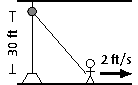
\includegraphics[scale=1.25]{figures/fig04_02_ex_12}
%
%Suppose the man stands directly next to the weight (i.e., a total rope length of 60 ft) and begins to walk away at a rate of 2ft/s. How fast is the weight rising when the man has walked:
%\begin{enumerate}
%\item	10 feet?
%\item	40 feet?
%\end{enumerate}
%How far must the man walk to raise the weight all the way to the pulley?
%
%\item Consider the situation described in Exercise \ref{exer:04_02_ex_12}. Suppose the man starts 40ft from the weight and begins to walk away at a rate of 2ft/s. 
%\begin{enumerate}
%\item	How long is the rope?
%\item	How fast is the weight rising after the man has walked 10 feet?
%\item	How fast is the weight rising after the man has walked 40 feet?
%\item	How far must the man walk to raise the weight all the way to the pulley?
%\end{enumerate}
%
%\item A company that produces landscaping materials is dumping sand into a conical pile. The sand is being poured at a rate of 5ft$^3$/sec; the physical properties of the sand, in conjunction with gravity, ensure that the cone's height is roughly 2/3 the length of the diameter of the circular base. 
%
%How fast is the cone rising when it has a height of 30 feet?
%
%\item A baseball diamond is a square with sides 90 feet long.  Suppose a baseball player is advancing from second to third base at the rate of 24 feet per second, and an umpire is standing on home plate.  Let  $\theta$ be the angle between the third baseline and the line of sight from the umpire to the runner.  How fast is $\theta$ changing when the runner is 30 feet from third base?
%	
%\item Sand is being dumped off a conveyor belt onto a pile in such a way that the pile forms in the shape of a cone whose radius is always equal to its height.  Assuming that the sand is being dumped at a rate of 10 cubic feet per minute, how fast is the height of the pile changing when there are 1000 cubic feet on the pile?
%	
%\item A swimming pool is 60 feet long and 25 feet wide. Its depth varies uniformly from 3 feet at the shallow end to 15 feet at the deep end, as shown below.
%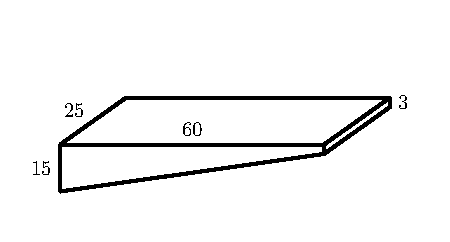
\includegraphics{figures/3_5_Ez3.eps}
%Suppose the pool has been emptied and is now being filled with water at a rate of 800 cubic feet per minute. At what rate is the depth of water (measured at the deepest point of the pool) increasing when it is 5 feet deep at that end?  Over time, describe how the depth of the water will increase:  at an increasing rate, at a decreasing rate, or at a constant rate.  Explain.
%
%\end{enumerate}
%
%%---------------------------------------------
%% END OF EXERCISES ON SECOND PAGE
%%---------------------------------------------
%\end{multicols*}
%\end{adjustwidth*}

\afterexercises